
\chapter{Realizability of Polygonal Linkages with Fixed Orientation\label{sec:hinge}}

\begin{thm}\label{thm:hinge2}
It is strongly NP-hard to decide whether a polygonal linkage whose hinge graph is a \textbf{tree} can be realized with fixed orientation.
\end{thm}

Our proof for Theorem~\ref{thm:hinge2} is a reduction from {\sc Planar-3-SAT} (P3SAT): decide whether a given Boolean formula in 3-CNF with a planar associated graph is satisfiable. The \emph{graph associated} to a Boolean formula in 3-CNF is a bipartite graph where the two vertex classes correspond to the variables and to the clauses, respectively; there is an edge between a variable $x$ and a clause $C$ iff $x$ or $\neg x$ appears in $C$. See Fig.~\ref{fig:assoc}(left).



\paragraph{The big picture.}
Given an instance $\Phi$ of P3SAT with $n$ variables and $m$ clauses, we construct a simply connected polygonal linkage $(\PP,H)$, of polynomial size in $n$ and $m$, such that $\Phi$ is satisfiable iff $(\PP,H)$ admits a realization with fixed orientation. We construct a polygonal linkage  in two main steps: First, we construct an auxiliary structure where some of the polygons have fixed position in the plane (called \emph{obstacles}), while other polygons are flexible, and each flexible polygon is hinged to an obstacle. Second, we modify the auxiliary construction into a polygonal linkage by allowing the obstacles to move freely, and by adding new polygons and hinges as well as an exterior \emph{frame} that holds the obstacle polygons in place. All polygons in our constructions are regular hexagons or long and skinny rhombi because these are the polygons that we can ``simulate'' with coin graphs in Section~\ref{sec:disk}.

We start with embedding the graph $A(\Phi)$ associated to $\Phi$ into a hexagonal tiling, and then replace the vertices by variable and clause gadgets, and the edges by transmitter gadgets (to be described below). A variable gadget corresponds to a cycle in the hexagonal tiling, a clause gadget to single vertex incident to three hexagons, and a transmitted gadget to a path along a sequence of edges and vertices of the tiling. Refer to Fig.~\ref{fig:assoc}(right).

The main idea for the auxiliary construction is the following. We thicken the edges of the hexagonal tiling into \emph{corridors} of uniform width, and the vertices of the tiling into regular triangles, which form \emph{junctions} between three corridors. The boundaries of the corridors form regular hexagons, which will be the obstacle polygons in our auxiliary construction. In each corridor, we insert flags, with one corner hinged to the boundary of the corridor. Each flag has two possible realizations (say, \emph{left} and \emph{right}) that can encode a binary variable: all flexible polygons turn in the same direction along a cycle (clockwise or counterclockwise) with suitable spacing between the hexagons (Fig.~\ref{fig:variable}(a-b)) and with a small flexible polygon at each junction (Fig.~\ref{fig:variable}(c)). Similarly, the value of a binary variable is transmitted via a chain of corridors and junctions. A clause of $\Phi$ is simulated by a single junction (Fig.~\ref{fig:clause}), where a small flexible polygon ensures that hexagons from at most two adjacent corridors enter the junction (i.e., at most two literals are false).

\paragraph{Auxiliary Construction: flags in a rigid frame.}
Let $\Phi$ be a Boolean formula in 3CNF with variables $x_1,\ldots , x_n$ and clauses $C_1,\ldots ,C_m$, and let $A(\Phi)$ be the associated planar graph. We modify $A(\Phi)$ to obtain a plane graph $\tilde{A}(\Phi)$ of maximum degree 3 as follows: Replace each \emph{variable} vertex $v$ by a cycle whose length equals the degree of $v$, and distribute the edges incident to $v$ among the vertices of the cycle.

Embed $\tilde{A}(\Phi)$ into the section of a hexagonal tiling (Fig.~\ref{fig:assoc}), contained in a regular hexagon of side length $N$, where $N$ is a polynomial of $n$ and $m$~\cite{BK+98}. Let $t=2N^3+1$ ($t$ will be the number of flags in a corridor). Scale the grid such that the cells become regular hexagons of side length $(5t-1)/2+\sqrt{3}$, and then scale each cell independently from its center to a hexagon of side length $(5t-1)/2$. These large hexagons are considered fixed obstacles in our auxiliary construction. Between two adjacent obstacle hexagons, there is a $\frac{5t-1}{2}\times \sqrt{3}$ rectangle, which we call a \emph{corridor}. Three adjacent corridors meet at a regular triangle, which we call a \emph{junction}. We next describe variable, clause, and transmitter gadgets.

\begin{figure}[htbp]
	\centering
	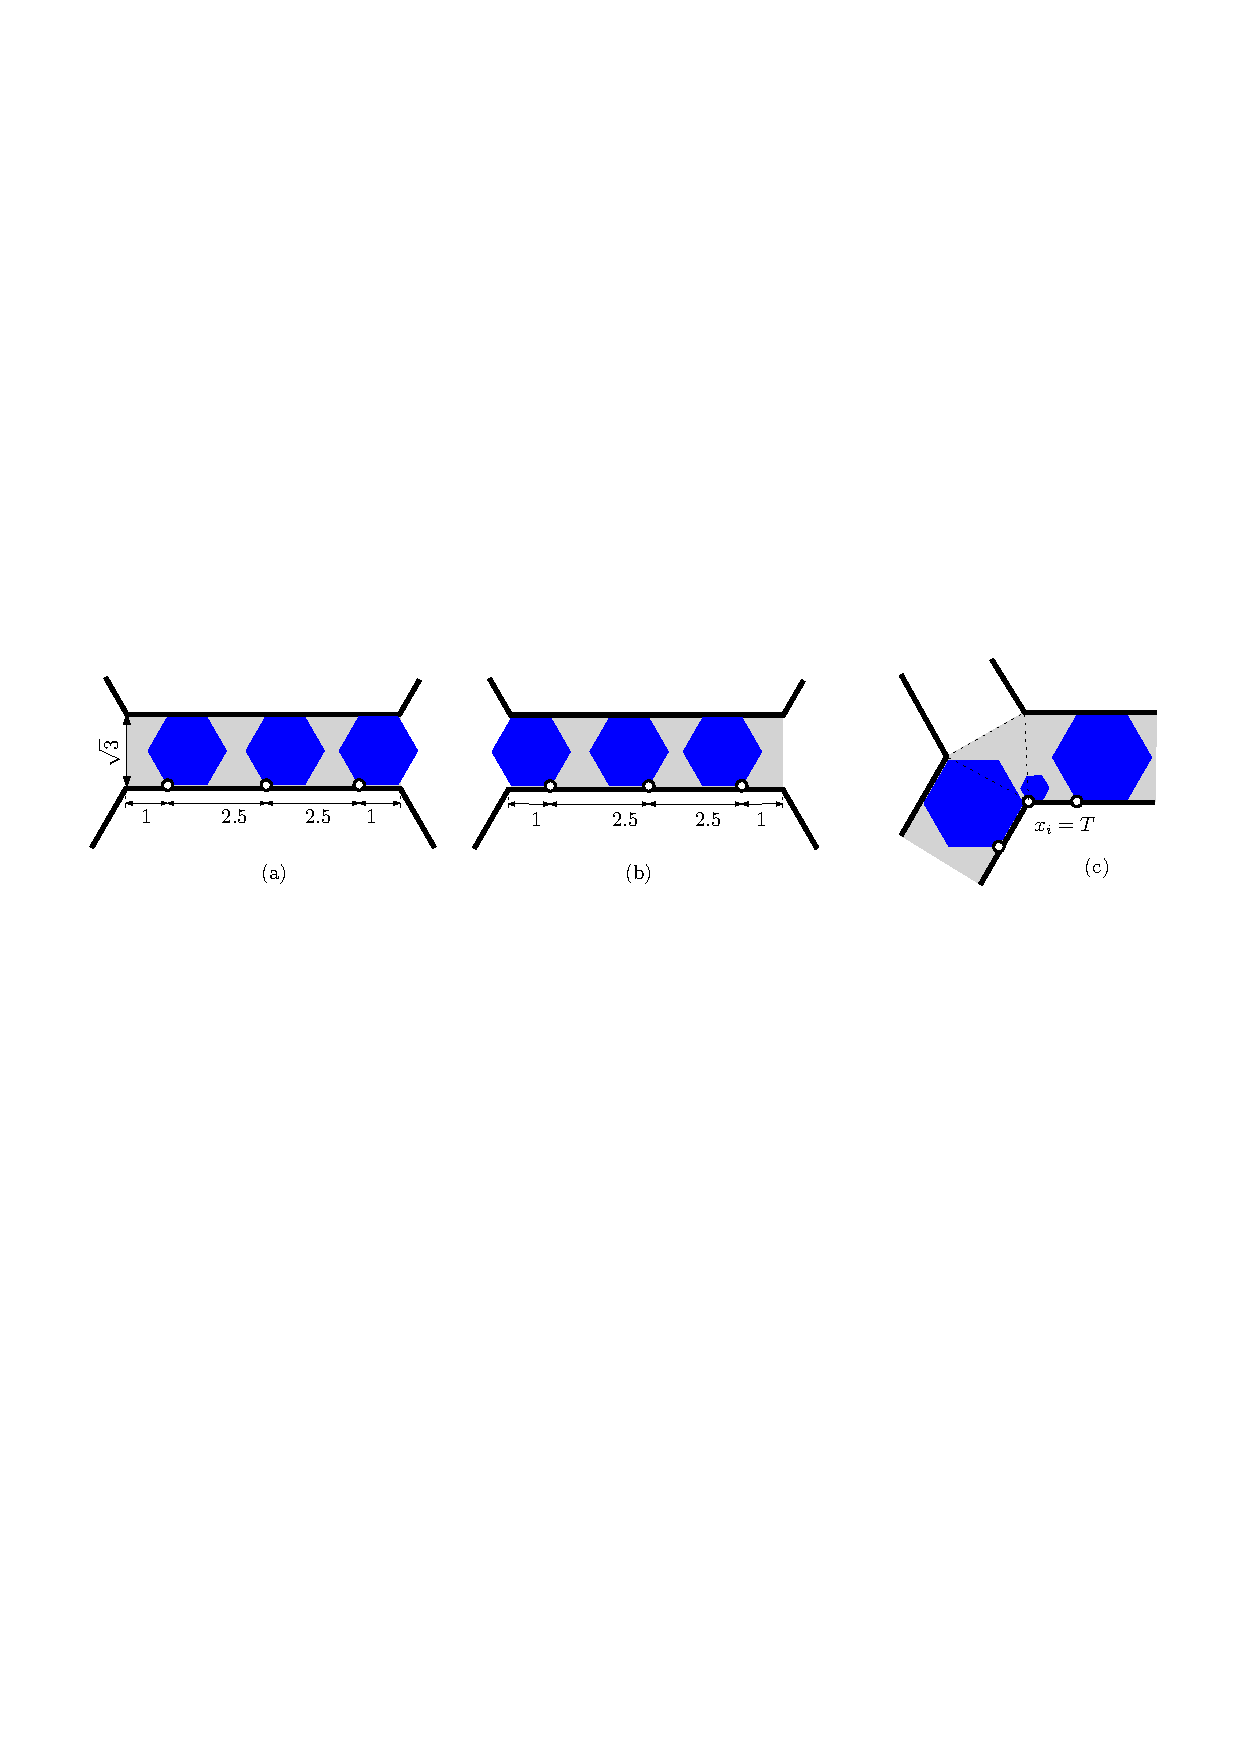
\includegraphics[width=0.9\columnwidth]{graphics/fig-variable-hex+}
	\caption{(a) A corridor when all unit hexagons are in state R.
(b) A corridor where all unit hexagons are in state L.
(c) A junction where a small hexagon between two corridors
    ensures that at most one unit hexagon enters the junction from those corridors.}
	\label{fig:variable}
\end{figure}

The basic building block of both variable and transmitter gadgets consists of $t$ regular hexagons of side length 1 (\emph{unit hexagons}, for short) attached to a wall of a corridor such that the hinges divide the wall into $t+1$ intervals of length $(1,2.5,\ldots ,2.5,1)$ as shown in Fig.~\ref{fig:variable}(a-b) for $t=3$. Since the height of the corridor is $\sqrt{3}$, each hexagon has exactly two possible realizations: it can lie either \emph{left} or \emph{right} of the hinge in a horizontal corridor. For simplicity, we use the same notation (R and L) in nonhorizontal corridors, too. Hence, the \emph{state} of each flag in a realization is either L or R. The following observation describes the key mechanism of a corridor.

\begin{observation}\label{obs:corridor}
\begin{itemize}
\item[]
\item[(1)] If the leftmost hexagon is in state R, then all $t$ hexagons are in state R, and the rightmost hexagon enters the junction on the right of the corridor.
\item[(2)] Similarly, if the rightmost hexagon is in state L, then all $t$ hexagons are in state L, and the leftmost hexagon enters the junction on the left of the corridor.
\end{itemize}
\end{observation}

Each junction is a regular triangle, adjacent to three corridors. In some of the junctions, we attach a small hexagon of side length $\frac{1}{3}$ to one or two corners of the junction (see Fig.~\ref{fig:variable}(c) and Fig.~\ref{fig:transmitter}). Importantly, if such a small hexagon is attached to a vertex between two corridors, then a unit hexagon can enter the junction from at most one of those corridors.

The {\bf variable gadget} for variable $x_i$ is constructed as follows. Recall that variable $x_i$ corresponds to a cycle in the associated graph $\tilde{A}(\Phi)$, which has been embedded as a cycle in the hexagonal tiling, with corridors and junctions. In each junction along this cycle, attach a small hexagon in the common boundary of the two corridors in the cycle. Observation~\ref{obs:corridor} and the small hexagons ensure that the state of any unit hexagon along the cycle determines the state of all other unit hexagons in the cycle. This property defines the binary variable $x_i$: If $x_i=T$, then all unit hexagons in the top horizontal corridors are in state R; and if $x_i=F$, they are all in state L.

\begin{figure}[htbp]
	\centering
	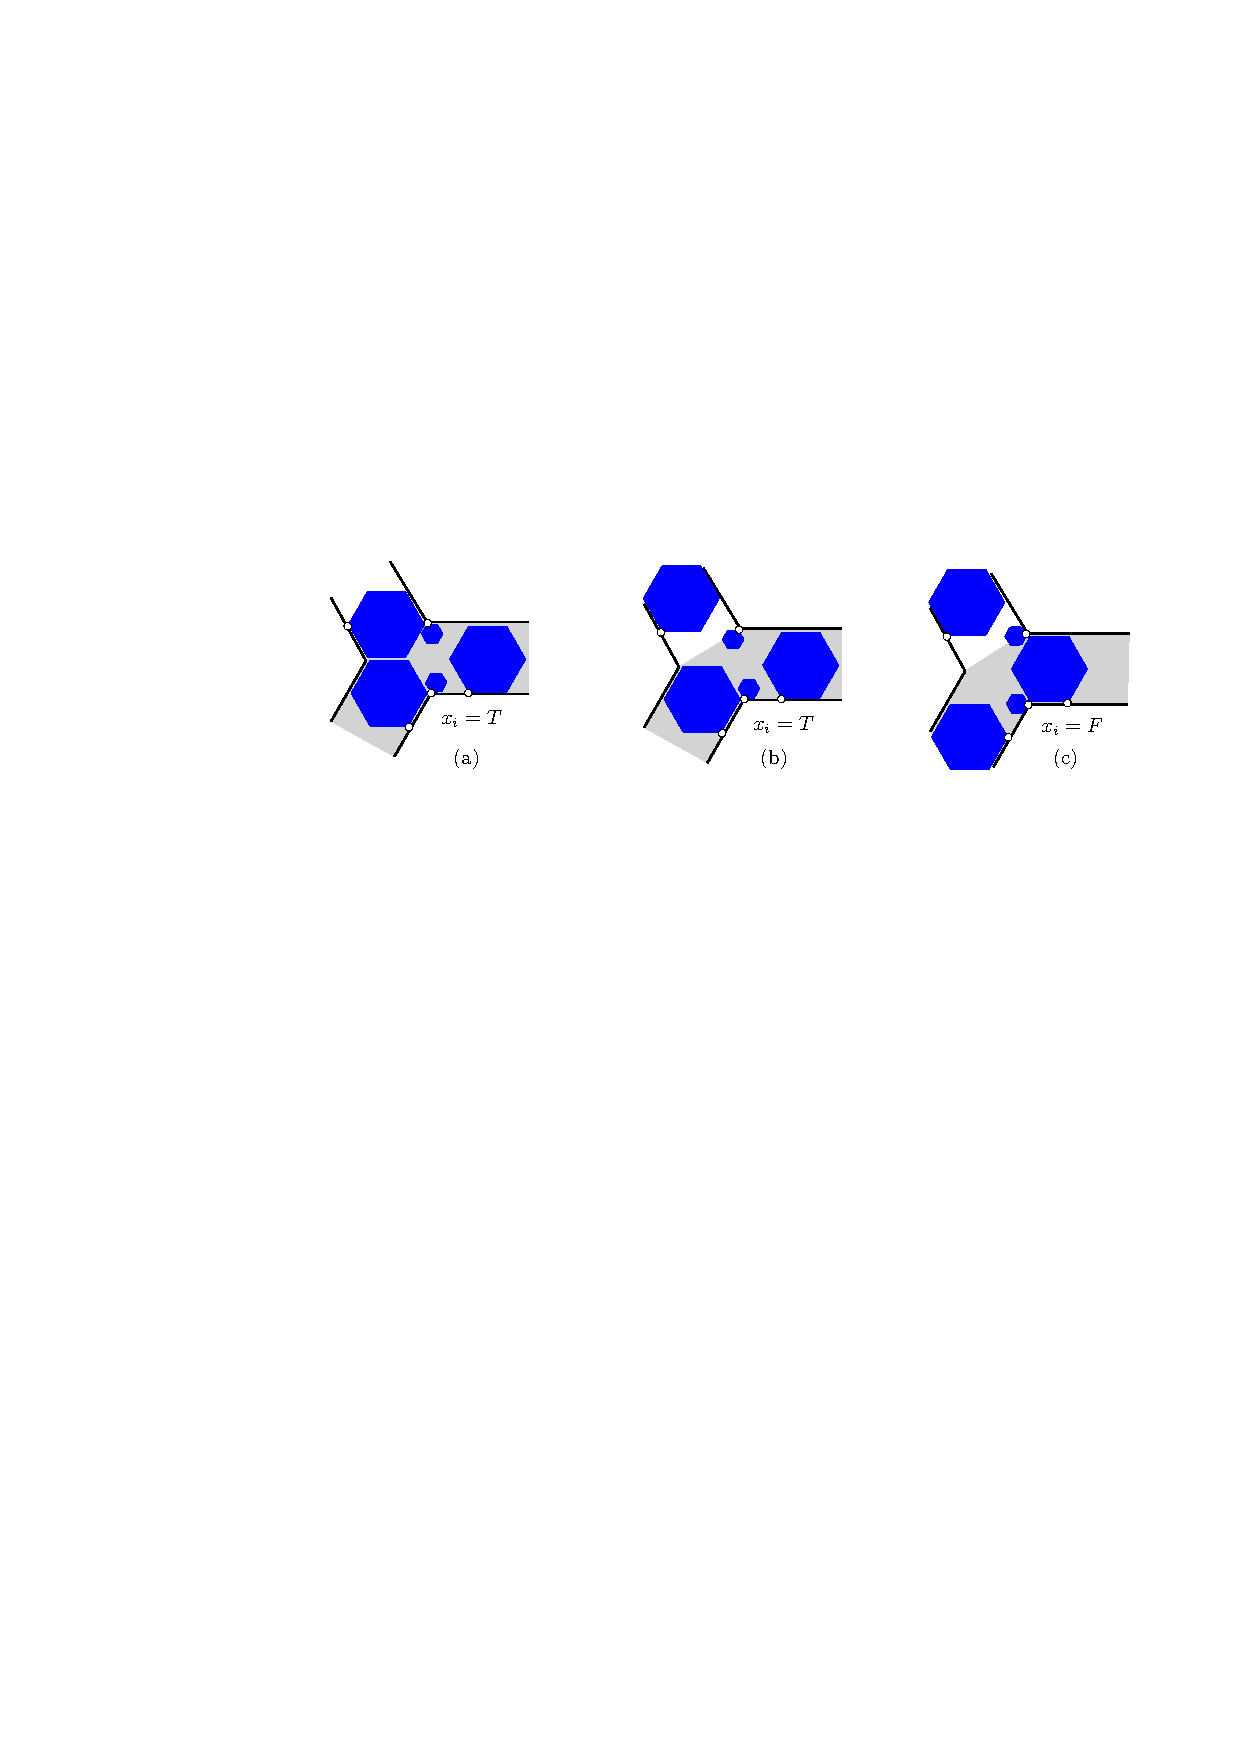
\includegraphics[width=0.7\columnwidth]{graphics/fig-transmitter-hex}
	\caption{The common junction of a variable gadget and a transmitter gadget.
(a) When $x_i=T$, a hexagon of the transmitter may enter the junction of the variable gadget.
(b) When $x_i=T$, the transmitter gadget has several possible realizations.
(c) When $x_i=F$, no hexagon from the transmitter enters a junction of the variable gadget.}
	\label{fig:transmitter}
\end{figure}

A {\bf transmitter gadget} is constructed for each edge $(x_i,C_j)$ of the graph $A(\Phi)$.
It connects a junction of the variable gadget $x_i$ with the junction representing the clause gadget $C_j$. The gadget consists of a path of corridors and junctions: at each interior junction, attach a small hexagon in the common boundary of the two corridors in the path (similarly to the variable gadget). At the common junction with the variable gadget $x_i$, we attach one additional small hexagon to one of the vertices (refer to Fig.~\ref{fig:transmitter}). If the literal $x_i$ (resp., $\overline{x}_i$) appears in $C_j$, then we attach a small hexagon to the corner of this junction such that if $x_i=F$ (resp., $\overline{x}_i=F)$, then the unit hexagon of the transmitter gadget cannot enter this junction. This ensures that false literals are always correctly transmitted to the clause junctions (and true literals can always transmit correctly).

The {\bf clause gadget} lies at a junction adjacent to three transmitter gadgets (see Fig.~\ref{fig:clause}). At such a junction, we attach a unit line segment to an arbitrary vertex of the junction, and a small hexagon of side length $\frac{1}{3}$ to the other end of the segment. If unit hexagons enter the junction from all three corridors (i.e., all three literals are false), then there is no space left for the small hexagon. But if at most two unit hexagons enter the junction (i.e., one of the literals is true), then the unit segment and the small hexagon are realizable.

\begin{figure}[htbp]
	\centering
	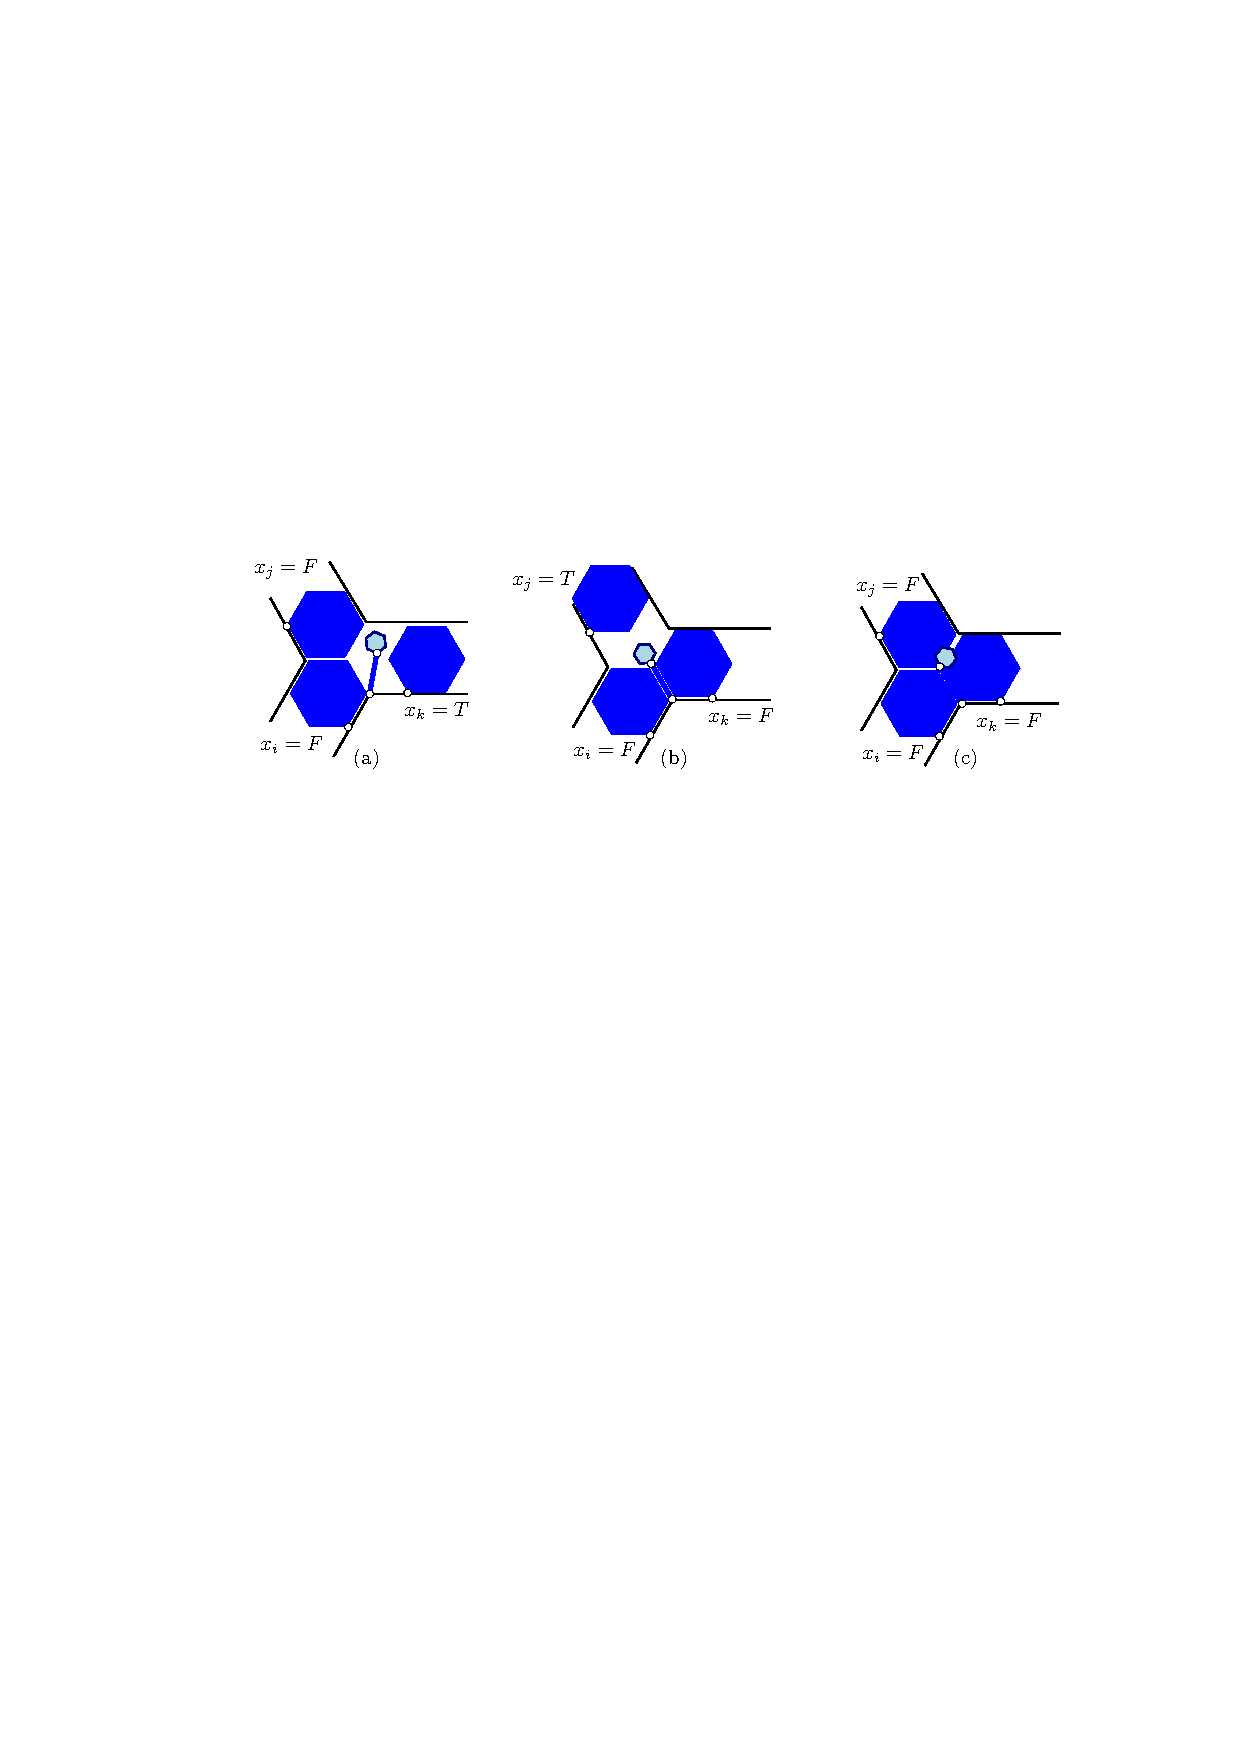
\includegraphics[width=0.7\columnwidth]{graphics/fig-clause-hex}
	\caption{(a-b) A clause gadget $(x_i\vee x_j\vee x_k)$ is
    realizable when at least one of the literals is {\sc True}.
    (c) The clause gadget cannot be realized when all three literals are {\sc False}.}
	\label{fig:clause}
\end{figure}

The following lemma summarizes our result about the auxiliary construction.
\begin{lem}\label{lem:aux}
For every instance $\Phi$ of P3SAT, the above polygonal linkage with flexible and obstacle polygons
has the following properties: (1) it has polynomial size; (2) its hinge graph is a forest;
(3) it admits a realization such that the obstacle polygons remain fixed if and only if $\Phi$ is satisfiable.
\end{lem}
The remaining details of our construction can be found in the full paper.
\section{Full Construction of the Reduction of Theorem~\ref{thm:hinge2}}
\label{app:full}
Let $\Phi$ be an instance of P3SAT (i.e., a Boolean formula $\Phi$
in 3-CNF with $n$ variables, $m$ clauses, and a planar graph $A(\Phi)$).
We construct a simply connected polygonal linkage $(\PP,H)$ that has a
realization with fixed orientation iff $\Phi$ is satisfiable.

We modify the auxiliary construction allowing all polygons to move freely, and by adding extra polygons and hinges so that the hinge graph becomes a \emph{tree}, and the size of the construction remains polynomial. Recall that our auxiliary construction is based on a polynomial section of the hexagonal tiling, using obstacle hexagons of side lengths $(5t-1)/2$, unit hexagons (of side length 1), and small hexagons of side length $\frac{1}{3}$. We modify it in 3 steps as follows.

\begin{enumerate}
\item Move the obstacle hexagons apart such that the width of each corridor increases from $\sqrt{3}$ to $\sqrt{3}+1/(100N)$.
\item Replace the unit segment in each the clause gadget by a skinny rhombus of diameter 1.1 and width $1/(200N)$.
\item Consider a large (polynomial-size) regular hexagon $R$ that contains all gadgets in our construction, and enclose $R$ by a \emph{frame} of 6 congruent regular hexagons, as shown in Fig.~\ref{fig:frame}(a), hinged together in a path.
\item Connect the frame and the obstacles in $R$ into a simply connected polygonal linkage: In each obstacle hexagon, the bottom or bottom-left side is adjacent to the frame or to a corridor. Introduce a hinge at the midpoint of one such side in each obstacle hexagon. If this side is adjacent to the frame, then attach the hinge to the frame. Otherwise, the hinge is attached to a new \emph{connector} polygon: a skinny rhombus of diameter 1 and width $1/(200N)$. The far corner of each rhombus is hinged to the unit hexagon in the middle of the corridor at shown in Fig.~\ref{fig:frame}(b).
\end{enumerate}

\begin{figure}[htbp]
	\centering
	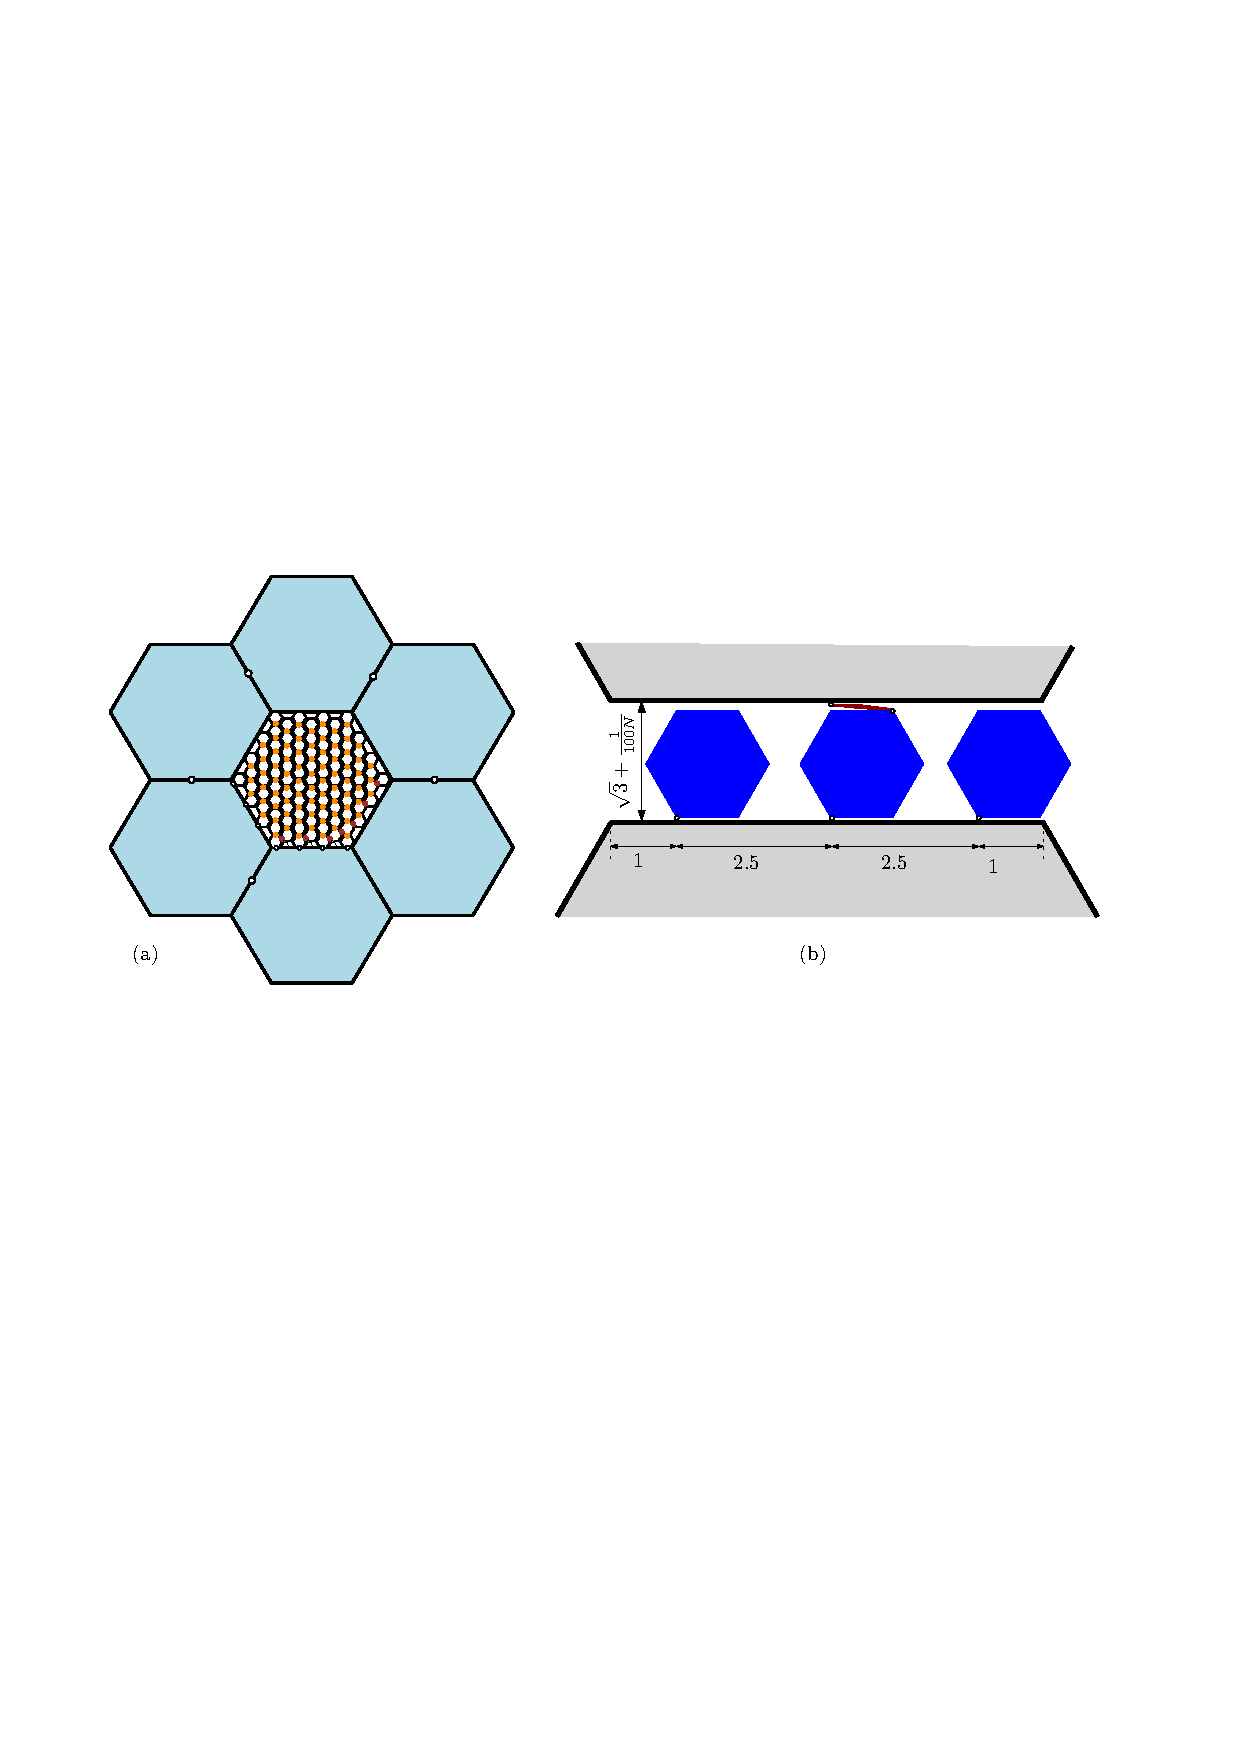
\includegraphics[width=0.95\columnwidth]{graphics/fig-frame-hex}
	\caption{(a) A frame (built of 6 hinged regular hexagons) encloses a hexagonal tiling, and
    vertical paths connect all obstacle hexagons to the frame.
    (b) A corridor is widened to $\sqrt{3}+1/N^2$. A connection between
    two adjacent obstacle hexagons is established via a skinny rhombus.}
	\label{fig:frame}
\end{figure}

We obtain a simply connected polygonal linkage. We now allow the ``obstacle'' hexagons
to move freely, and call their original fixed position \emph{canonical}. We may assume
w.l.o.g. that the frame is at its original position. It is enough to show that the obstacle
hexagons are still confined to an $1/N$-neighborhood of their canonical position, then it
follows that the polygonal linkage is realizable if and only if $\Phi$ is satisfiable.

The obstacle hexagons in the bottom and bottom-left rows are hinged directly to the frame,
and so they are locked in their canonical position. Consider two obstacle hexagons on opposite
sides of a corridor with connector. The distance between the midpoints of the opposite sides of
the corridor is at least $\sqrt{3}$ (due to the unit hexagons in the corridor) and at most
$1+\sqrt{3}$ (due to the connector polygon). The length of the corridor is much larger,
$(5t-1)/2=5N^3+2$, so the orientations of the two adjacent obstacles differ by at most $1/2N^3$.
Consequently, the orientation of \emph{any} obstacle differs from canonical by at most $1/2N^2$.
Due to the unit hexagons within the horizontal corridors, the length of any vertical segment between
the opposite sides of a horizontal corridor is at least $1-1/N^2$. The vertical distance between the
bottom and top sides of the frame gives an upper bound of  $2N/(100N^2)=1/(50N)$ for the sum of these
vertical distances. We conclude that the $y$-coordinates of the obstacles are within $1/(10N)$
of the canonical position. Due to the connector polygons, the $x$-coordinates of
two adjacent obstacles differ by either less than the vertical offset or by about
one unit. However, the horizontal distance between the left and right frames prevent
a shift of this magnitude. So the $x$-coordinates of the obstacle hexagons are also
within $1/N$ of the canonical position.


